\documentclass[11pt,a4paper]{report}

\usepackage[french]{babel}
\usepackage[utf8]{inputenc}
\usepackage[T1]{fontenc}
\usepackage{geometry}
\usepackage{graphicx}
\usepackage{tabularx}
\usepackage{booktabs}
\usepackage{hyperref}
\usepackage{titlesec}
\usepackage{setspace}
\usepackage{fancyhdr}

\geometry{margin=2.5cm,headheight=43pt,headsep=18pt,footskip=24pt}

\setlength{\parindent}{0pt}
\setlength{\parskip}{0.6em}

\titleformat{\chapter}{\Huge\bfseries}{\thechapter}{1em}{}
\titleformat{\section}{\Large\bfseries}{\thesection}{0.8em}{}

\hypersetup{
colorlinks=true,
linkcolor=black,
urlcolor=blue
}

\pagestyle{fancy}
\fancyhf{}
\fancyhead[C]{\begin{tabular}{c}Scanner 3D\\Cahier des charges fonctionnel - V2\end{tabular}}
\fancyfoot[L]{11.03.2026}
\fancyfoot[R]{\thepage}
\renewcommand{\headrulewidth}{0.4pt}
\renewcommand{\footrulewidth}{0.4pt}

\fancypagestyle{plain}{
\fancyhf{}
\fancyhead[C]{\begin{tabular}{c}Scanner 3D\\Cahier des charges fonctionnel - V2\end{tabular}}
\fancyfoot[L]{11.03.2026}
\fancyfoot[R]{\thepage}
\renewcommand{\headrulewidth}{0.4pt}
\renewcommand{\footrulewidth}{0.4pt}
}

\begin{document}

%------------------------------------------------
% PAGE DE GARDE
%------------------------------------------------

\begin{titlepage}

\centering

\vspace*{0.5cm}
\begin{minipage}{0.45\textwidth}
\centering

\includegraphics[height=1.8cm]{logo_heig.png}
\end{minipage}
\hfill
\begin{minipage}{0.45\textwidth}
\centering

\includegraphics[height=1.8cm]{logo_hesso.pdf}
\end{minipage}

\vspace{2.2cm}

{\Huge\bfseries Scanner 3D}

\vspace{0.5cm}

{\Large Cahier des charges fonctionnel}

\vspace{0.3cm}

{\large Version 2}

\vspace{2cm}

{\Large Projets Multidisciplinaires 2026}

\vfill

\begin{tabular}{rl}
\textbf{Rédigé par :} & Berthoud Tom, EAI \\
& Jason Weber, EAI \\
& Hadrien Fuentes, EAI \\
& Luc Marchand, EAI \\
& Tim Stamm, ROCM \\
\\
\textbf{Professeur répondant :} & Bornand Cédric
\end{tabular}

\vfill

HEIG-VD \\
Route de Cheseaux 1 \\
1401 Yverdon-les-Bains

\end{titlepage}

%------------------------------------------------
% HISTORIQUE
%------------------------------------------------

\section*{Historique du document}

\begin{center}
\begin{tabularx}{0.8\textwidth}{c c X}
\toprule
\textbf{Version} & \textbf{Date} & \textbf{Changements} \\
\midrule
V1 & 04.03.2026 & Version initiale \\
V2 & 11.03.2026 & Version révisée (exigences de précision clarifiées et mesurables) \\
\bottomrule
\end{tabularx}
\end{center}

%------------------------------------------------
% RÉFÉRENCES
%------------------------------------------------

\section*{Références normatives}

Les documents suivants cités dans le texte constituent, pour tout ou partie de leur contenu, des exigences du présent document.

\begin{center}
\begin{tabularx}{\textwidth}{l X}
\toprule
\textbf{Norme} & \textbf{Description} \\
\midrule
ISO/IEC Dir 2 : 2016 & Principes et règles de structure et de rédaction des documents ISO et IEC \\
OMG UML 2.5.1 & Unified Modeling Language pour l’ingénierie logicielle \\
\bottomrule
\end{tabularx}
\end{center}

%------------------------------------------------
% ABRÉVIATIONS
%------------------------------------------------

\section*{Abréviations}

Cette section de termes et définitions précise les terminologies techniques et autres acronymes propres au projet.

\begin{center}
\begin{tabularx}{0.7\textwidth}{l X}
\toprule
\textbf{Terme} & \textbf{Définition} \\
\midrule
HEIG-VD & Haute École d’Ingénierie et de Gestion du Canton de Vaud \\
MakeLab & Laboratoire de prototypage et de fabrication de l'HEIG-VD \\
\bottomrule
\end{tabularx}
\end{center}

\tableofcontents

\newpage

%------------------------------------------------
% INTRODUCTION
%------------------------------------------------

\chapter{Introduction}

Le projet consiste à concevoir et réaliser une boîte de scan permettant de mesurer les dimensions d’un objet tridimensionnel et de les convertir en un modèle numérique exploitable.

L’objectif est de développer un prototype fonctionnel capable de générer un nuage de points ou un modèle 3D simplifié, exportable dans un format numérique adapté. Ce dispositif sera destiné au MakeLab de la HEIG-VD afin d’offrir aux étudiants et collaborateurs un outil accessible pour la numérisation d’objets.

\section{Contexte}

Ce projet s’inscrit dans le cadre des activités de développement et d’innovation du MakeLab de la HEIG-VD, qui vise à mettre à disposition des outils technologiques facilitant la conception, le prototypage et la fabrication numérique.

La réalisation de cette boîte de scan répond au besoin croissant de solutions simples et accessibles pour la numérisation 3D d’objets, notamment dans un contexte pédagogique et expérimental.

%------------------------------------------------
% PROBLÈME
%------------------------------------------------

\chapter{Description du problème}

Dans le cadre d’un projet multidisciplinaire, nous avons proposé de créer une solution de numérisation 3D destinée au MakeLab de la HEIG-VD. L’objectif est de développer une boîte de scan capable de mesurer un objet et de générer un modèle numérique exploitable.

Les solutions existantes étant souvent coûteuses ou complexes, le projet vise à proposer un système accessible, simple d’utilisation et adapté à un environnement pédagogique.

Le dispositif reposera sur l’utilisation d’un laser et d’une caméra afin de reconstruire la géométrie de l’objet par triangulation.

Le but est d’installer une solution fonctionnelle au MakeLab, utilisable par les étudiants et collaborateurs.

%------------------------------------------------
% ANALYSE DU BESOIN
%------------------------------------------------

\chapter{Analyse du besoin}

Avant toute chose, nous devons identifier les utilisateurs principaux. Dans le cas du scanner, les utilisateurs identifiés sont ceux qui ont accès au MakeLab :

\begin{itemize}
\item Étudiant ingénieur
\item Collaborateur
\item Professeur dans le domaine de l’ingénierie
\end{itemize}

\section*{Besoins identifiés}

\begin{center}
\begin{tabularx}{\textwidth}{c X}
\toprule
\textbf{\#} & \textbf{Besoins} \\
\midrule
1 & Obtenir un fichier objet à partir d’une pièce simple (au moins un type parmi les suivants : STL, OBJ) \\
2 & Scanner les faces latérales visibles \\
3 & Temps de prise en main inférieur à 10 minutes \\
4 & Temps de scan inférieur à 10 minutes \\
5 & Scanner une pièce de dimension 15\,cm × 15\,cm × 15\,cm \\
6 & Système automatisé \\
\bottomrule
\end{tabularx}
\end{center}

\begin{center}
\textit{Tableau 1 : Analyse des besoins des utilisateurs}
\end{center}

%------------------------------------------------
% FONCTIONS
%------------------------------------------------

\chapter{Fonctions et exigences du système}

\section{Fonctions de service}

\begin{center}
\begin{tabularx}{\textwidth}{c X c X}
\toprule
 & \textbf{Fonctions de service} &  & \textbf{Exigences} \\
\midrule
FS1 & Automatiser le processus de scan de pièce 3D & E1 & Système complètement automatisé \\
\midrule
FS2 & Scanner la pièce & E2 & Mesurer la géométrie par un système optique \\
\midrule
FS3 & Zone de scan & E3 & Pièce de dimension 150 × 150 × 150 mm \\
\midrule
FS4 & Donner un retour visuel à l’utilisateur en cas d’erreur ou de fin de cycle & E5 & LEDs / écran \\
\midrule
FS5 & Générer un modèle 3D & E6 & Produire un fichier au format STL ou OBJ \\
\midrule
FS6 & Simple à utiliser & E7 & Prise en main $\leq 10$ min pour un utilisateur novice et scan complet sans assistance dans $\geq 90\%$ des cas (n=10) \\
\bottomrule
\end{tabularx}
\end{center}

\section{Fonctions techniques}

\begin{center}
\begin{tabularx}{\textwidth}{c X c X}
\toprule
 & \textbf{Fonctions techniques} &  & \textbf{Exigences} \\
\midrule
FT1 & Mettre en place une boîte fermée pour le système de mesure & E9 & Limiter l'éclairage parasite dans la zone de scan. \\
\midrule
FT2 & Mettre en place un moyen de communication & E10 & USB et/ou interface web \\
\midrule
FT3 & Créer une interface utilisateur & E11 & Lancer un scan en $\leq 5$ actions depuis l'écran d'accueil et afficher les états: prêt, scan en cours, terminé, erreur \\
\midrule
FT4 & Capturer les images du laser déformé sur l’objet & E12 & Utiliser une caméra positionnée avec un angle connu \\
\midrule
FT5 & Traiter les données numériquement & E13 & Développer un programme permettant le traitement, le filtrage et l’export \\
\midrule
FT6 & Réglage des paramètres géométriques & E14 & Permettre la calibration des paramètres de scan \\
\midrule
FT7 & Gérer le mouvement de l’objet scanné & E15 & Intégrer un plateau rotatif motorisé \\
\bottomrule
\end{tabularx}
\end{center}

\section{Fonctions de contrainte}

\begin{center}
\begin{tabularx}{\textwidth}{c X c X}
\toprule
 & \textbf{Fonctions de contrainte} &  & \textbf{Exigences} \\
\midrule
FC1 & Respecter le budget & E16 & Budget inférieur ou égal à 300 CHF \\
\midrule
FC2 & Garantir la sécurité des utilisateurs & E17 & Utiliser des matériaux non toxiques pour toutes les pièces accessibles et garantir des arêtes non tranchantes \\
 &  & E18 & Rendre inaccessibles les pièces en mouvement pendant le scan \\
 &  & E19 & Isoler le rayon laser de l'utilisateur, avec coupure automatique à l’ouverture de la boîte \\
\midrule
FC3 & Être compatible avec l'environnement du MakeLab & E20 & Fonctionner sur une alimentation standard de 230 V \\
 &  & E21 & Respecter un encombrement maximal de 500 $\times$ 500 $\times$ 500 mm et une masse totale $\leq 15$ kg \\
\midrule
FC4 & Respecter les délais du projet & E22 & Disposer d’un prototype fonctionnel livré au plus tard le 7 juin 2026 \\
\midrule
FC5 & Limiter le périmètre aux pièces simples & E23 & Scanner des objets sans cavité fermée, sans contre-dépouille $>45^\circ$, et de taille $\leq 150$ mm par axe \\
\midrule
FC6 & Garantir une précision et une répétabilité mesurables & E24 & Atteindre une erreur absolue moyenne $\leq 2$ mm et une répétabilité (écart-type) $\leq 1$ mm sur 3 scans successifs du même objet de référence \\
\bottomrule
\end{tabularx}
\end{center}

%------------------------------------------------
% DIAGRAMME FAST
%------------------------------------------------

\chapter{Diagramme FAST}

Le diagramme FAST ci-dessous synthétise la logique fonctionnelle du système à partir des fonctions de service, des fonctions techniques et des principales contraintes identifiées dans ce cahier des charges.

\begin{figure}[h]
\centering
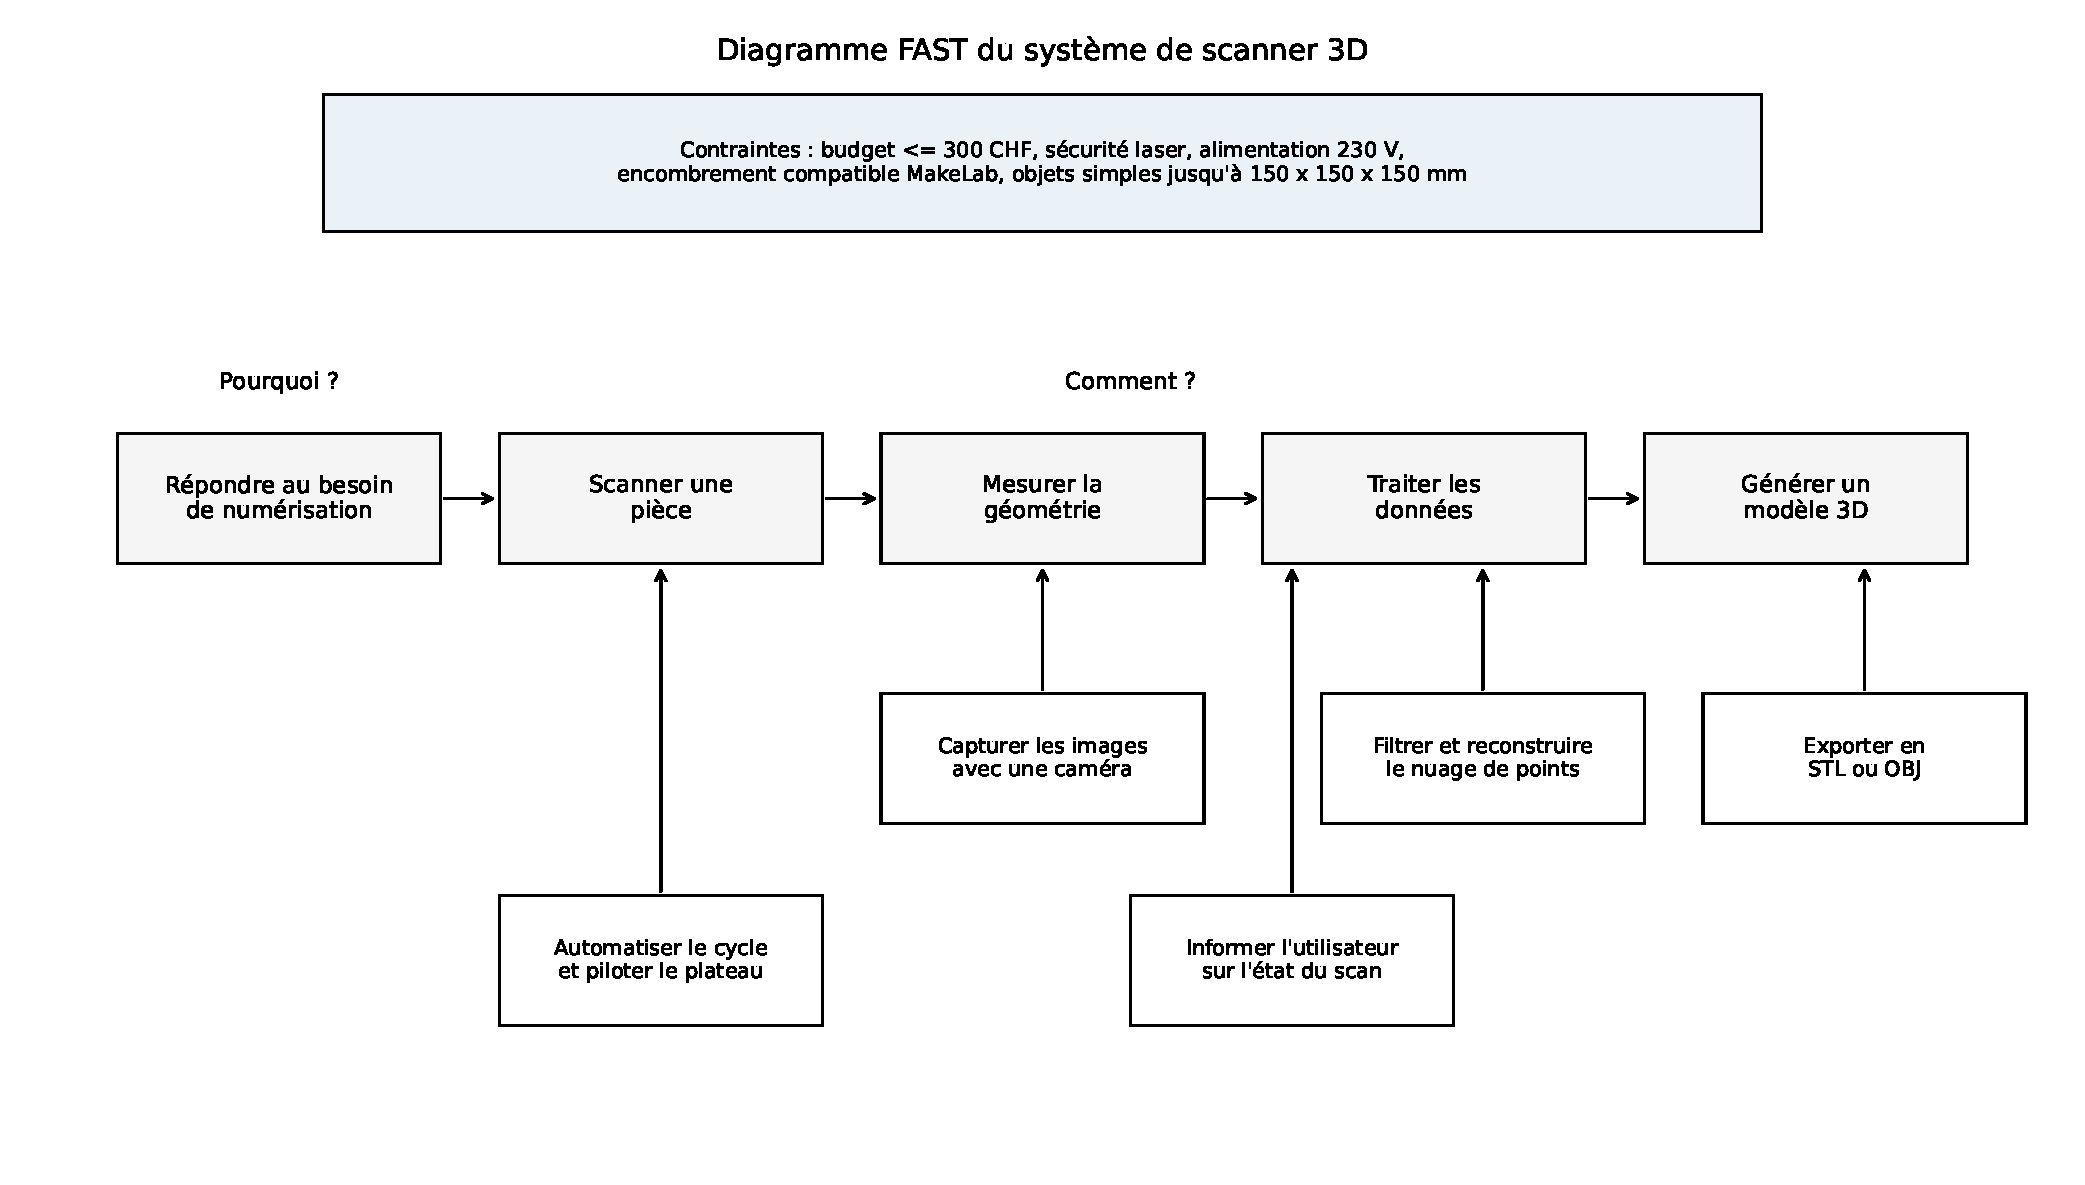
\includegraphics[width=\textwidth]{fast_diagram.pdf}
\caption{Diagramme FAST du scanner 3D}
\end{figure}

%------------------------------------------------
% BIBLIOGRAPHIE
%------------------------------------------------

\chapter{Bibliographie}

\section*{Webographie}

OpenScan. \textit{OpenScan - 3D Scanner}. Documentation officielle du projet OpenScan. Disponible sur : \url{https://openscan-org.github.io/OpenScan-Doc/}

OpenScan. \textit{OpenScan Mini}. Documentation matérielle du scanner OpenScan Mini. Disponible sur : \url{https://openscan-org.github.io/OpenScan-Doc/hardware/OpenScanMini/}

OpenScan. \textit{3D Scan Quality}. Exemples et discussion sur la qualité des scans obtenus. Disponible sur : \url{https://openscan-org.github.io/OpenScan-Doc/photogrammetry/quality/}

\section*{Outil d'assistance à la recherche}

OpenAI. \textit{ChatGPT}. Outil conversationnel utilisé ponctuellement pour explorer des pistes techniques, comparer des approches existantes et formuler certaines questions de cadrage. Consulté en mars 2026. Disponible sur : \url{https://openai.com/chatgpt/overview/}

%------------------------------------------------
% ANNEXES
%------------------------------------------------

\chapter{Annexes}

\end{document}
